

%\documentclass{acm_proc_article-sp}
%\documentclass{sig-alternate}
\documentclass[conference]{IEEEtran}
\usepackage{multirow}
\usepackage{fancyheadings}
\usepackage{algorithmic}
\usepackage{amssymb}
\usepackage{amsmath}
\usepackage{xspace}
\usepackage{pslatex}
\usepackage{microtype}
\usepackage{subfigure}
\usepackage{indentfirst}
\usepackage{listings, algorithm, algorithmic, graphicx, listing}
\usepackage{relsize}
\usepackage{multicol}
\usepackage{flushend}

%\usepackage{todonotes}
\input{macros}

% % Add line between figure and text
 %\makeatletter
 %\def\topfigrule{\kern3\p@ \hrule \kern -3.4\p@} % the \hrule is .4pt high
 %\def\botfigrule{\kern-3\p@ \hrule \kern 2.6\p@} % the \hrule is .4pt high
 %\def\dblfigrule{\kern3\p@ \hrule \kern -3.4\p@} % the \hrule is .4pt high
 %\makeatother

 % If there is a line, you can get away with reducing the separation between
 % figures and text.  Don't do this without the line, though.
 \addtolength{\textfloatsep}{-.5\textfloatsep}
 \addtolength{\dbltextfloatsep}{-.5\dbltextfloatsep}
 \addtolength{\floatsep}{-.5\floatsep}
 \addtolength{\dblfloatsep}{-.5\dblfloatsep}

% Left and right curly braces in tt font
\newcommand{\ttlcb}{\texttt{\char "7B}}
\newcommand{\ttrcb}{\texttt{\char "7D}}

\newcommand{\totaloc}{99458 }
\newcommand{\subnum}{10 }
\newcommand{\warnings}{22 }
\newcommand{\bugs}{12 }
\newcommand{\newbugs}{7 }
\newcommand{\falses}{10 }
\newcommand{\annotationnum}{7 }
\newcommand{\filternum}{11 }

% \newcommand{\smallstep}{\vspace{-2mm}}
% \newcommand{\tinystep}{\vspace{-1mm}}
\newcommand{\smallstep}{\relax}
\newcommand{\tinystep}{\relax}


\newenvironment{myindentpar}[1]%
{\begin{list}{}%
         {\setlength{\leftmargin}{#1}}%
         \item[]%
}
{\end{list}}


% Reduce indentation in lists.
%\setlength{\leftmargini}{.5\leftmargini}

%% Bring items closer together in list environments
%% This doesn't work with an optional argument to the list environment.
% Prevent infinite loops
\let\Itemize =\itemize    
\let\Enumerate =\enumerate
\let\Description =\description
% Zero the vertical spacing parameters
\def\Nospacing{\itemsep=0pt\topsep=0pt\partopsep=0pt\parskip=0pt\parsep=0pt}
% Redefine the environments in terms of the original values
\renewenvironment{itemize}{\Itemize\Nospacing}{\endlist}
\renewenvironment{enumerate}{\Enumerate\Nospacing}{\endlist}
\renewenvironment{description}{\Description\Nospacing}{\endlist}

%\newcommand{\todo}[1]{{TODO #1}}
\newcommand{\todo}[1]{{\color{red}\bfseries [[{#1}]]}}
\newcommand{\sai}[1]{{\color{blue}\todo{for Sai: #1}}}
\newcommand{\yuyin}[1]{{\color{red}\todo{for Yuyin: #1}}}

\newcommand{\ourtool}{SQLSynthesizer\xspace}

\newcommand{\allex}{23\xspace}

\newcommand{\exnum}{23\xspace}
\newcommand{\solexnum}{15\xspace}

\newcommand{\pnum}{5\xspace}
\newcommand{\solpnum}{5\xspace}

\newcommand{\respnum}{12\xspace}

\newcommand{\avgtime}{8\xspace}
\newcommand{\avgsucctime}{9\xspace}
\newcommand{\avground}{XXX\xspace}
\newcommand{\avgsuccround}{2.3\xspace}

\newcommand{\avghum}{XX\xspace}
\newcommand{\avgsucchum}{3.6\xspace}
\newcommand{\avgtuple}{XXX\xspace}
\newcommand{\avgsucctuple}{22\xspace}

\newcommand{\yes}{\textbf{Y}\xspace}
\newcommand{\no}{\textbf{N}\xspace}
\newcommand{\xx}{\textbf{X}\xspace}

\begin{document}

\title{Automatically Synthesizing SQL Queries from \\Input-Output Examples}



\author{\IEEEauthorblockN{Sai Zhang\quad Yuyin Sun}
\IEEEauthorblockA{Computer Science \& Engineering\\
University of Washington, USA\\
\{szhang, sunyuyin\}@cs.washington.edu}}


\maketitle

\begin{abstract}

Many computer end-users, such as
research scientists and business analysts, need to frequently query
a database, yet lack the programming knowledge to do such tasks smoothly.
To alleviate this problem, we present
a \textit{programming by example} technique
(and its tool implementation, called \ourtool)
to help end-users automate such query tasks.
\ourtool takes from users an input and output example of how the
database should be queried, and then synthesizes a SQL query that
reproduces the example output from the example input.
Later, when the synthesized
SQL query is applied to another, potentially larger, database with a
similar schema as the example input, the synthesized SQL query produces
a corresponding result that is similar to the example output. 


%\todo{num is missing here}
We evaluated \ourtool on \exnum SQL exercises from a classic
database textbook and \pnum SQL questions raised by
real-world users from online forums.
\ourtool infers correct queries for \solexnum textbook
exericses and \solpnum forum questions, including one question
that received no replies.
\end{abstract}



%\vspace{-1mm}

\section{Introduction}
\label{sec:introduction}


The big data revolution over the past few years has resulted
in significant advances in digitization of massive amounts
of data and accessibility of computational devices to massive
proportions of the population. A key challenge faced by many
enterprise or computer end-users nowadays is the management
of their increasingly large and complex databases.
%, which can contain
%hundreds and even thousands of tables. 


%but they often need to
%query databases to obtain relevant data to support their business decisions.


%\subsection{End-users' Difficulties in Writing SQL Queries}
\vspace{1mm}
\noindent \textbf{\textit{Motivation.}}
Although the relational database management system (RDBMS) and the
de facto language (SQL) are perfectly adequate for most end-users'
needs~\cite{Howe:2011}, the costs associated with deployment and
use of database software and SQL are prohibitive. 
For example, as pointed out in~\cite{Gray:2005},
conventional RDBMS software remains underused
in the long tail of science: the large number of users, such as the
research scientists who are in relatively small labs and individual
researchers, have limited IT training, staff and infrastructure yet
collectively produce the bulk of scientific knowledge. 

The problem is exacerbated by the fact that many end-users
have myriad diverse backgrounds including research scientists,
business analysts, commodity traders, human resource managers,
finance professionals, and marketing managers. 
Those end-users are not professional programmers, but are experts in some
other domains. They need to query a variety of information on their
database and use the information to support their business decisions.
Although most end-users can clearly describe \textit{what} the task is, they
are often stucked with the process of \textit{how} to
write a desirable database query even after
receiving step-by-step, detailed,
and syntactically correct instructions.
Thus, many end-users often need to
seek information from online help forums, or ask
SQL experts. This process can be repetative, laborious, and frustrating.
To assist end-users in performing database query tasks,
%For them, they need an \textit{intelligent} tool
%to assist them to perform database query tasks. 
a highly accessible tool that can be used to ``describe''
their needs and connect their intentions to executable
SQL queries would be highly desirable.

%simply can not get the SQL query correct,
%either due to the syntax complexity of the SQL language itself,
%or the structure complexity of the databases.
%To write a correct SQL query, end-users often need to
%seek information from online help forums, or ask
%SQL experts. This process can be repetative, laborious, and frustrating.

%However, such practice is inefficient and time-consuming.
%Non-professional end-users 


%\todo{move the following sentence to somewhere esle}

%Similarly, other end-users
%such as business analysts who query databases frequently often
%do not have significant SQL expertise.

%To learn how to query a RDBMS, most end-users often refer
%to a textbook or online resources to first get familiar with
%the basic idioms of the SQL language. Then, they may
%try to write some experimental queries, execute them
%on a sample database to observe the output, and
%subsequently revise the queries (if the output is not desirable).

%The above process may
%predicates in the \CodeIn{where} clause,
%tables in the \CodeIn{from} clause, or columns in the \CodeIn{select} clauses.



%\subsection{Existing Solutions}

\vspace{1mm}
\noindent \textbf{\textit{Existing Solutions.}}
\textit{Graphical User Interfaces} (GUIs) and \textit{general programming languages}
are two state-of-the-art approaches in helping end-users perform
database queries. However, both approaches are far from satisfactory.

Many RDBMS come with a well-designed GUI with tons of features.
However, 
%as a database management system often comes with tons
%of features, end-users struggle to find the correct feature or
%succession of commands to use from a maze of features to accomplish
%their tasks.
a GUI is often fixed, and does not permit users to personalize
a database's functionality for their query tasks. On the other hand,
as a GUI supports more and more customization features, users
may struggle to discover those features, which can significantly
degrade its usability. 

General programming languages, such as SQL,
Java (with JDBC), or other domain specific query languages, 
serve as a fully expressive medium  for
communicating a user's intention to a database. However, 
general purpose programming languages have never been easy for
end-users who are not professional programmers.  Learning
a practical programming language (even a simplified, high-level domain
specific language, such as MDX~\cite{mdx}) often requires a substantial amount
of time and energy that a typical end-user would not prefer,
and should not be expected, to invest. 



%\subsection{Synthesizing SQL Queries from Input-Output Examples}

%After carefully studying how end-users were describing their
%encountered SQL query problems on online help forums, we observed that
%one of the most common ways for end-users to
%express their intents is using input-output examples. 

\vspace{1mm}
\noindent \textbf{\textit{Our Solution: Synthesizing SQL Queries from Input-Output Examples}}
In this paper, we present a technique (and its tool
implementation, called \ourtool) to automatically synthesize SQL queries
from input-output examples. Although input-output examples may lead to
underspecification, writing them, as opposed to writing
declarative sepcifications or imperative code
of any form, is one of the most straightforward ways
to describe \textit{what} the task is.
%\ourtool takes example input
%table(s) and output table from the end-users, and then automatically
%infers a SQL query (or multiple queries, if exist) that queries
%against the input tables and returns the output example.
If the sythesized SQL query is applied
to the example input, then it produces the example output; and if the
SQL query is applied to other similar inputs (potentially much larger tables),
then the SQL query produces a corresponding output.


%\ourtool uses such input-output examples
%as a natural interface to "understand" an end-user's intention
%and provide corresponding assistance.

%Compared with other alternatives (such as, writting
%a declarative specification) to specify a user's intention,
%input-output examples, although may lead to underspecification,
%serve as a more straightforward way  is and a natural interface that a tool can provide assistance.

\ourtool is designed to be used by non-expert database
end-users when they do not know how
to write a desirable SQL query. 
End-users can use \ourtool to obtain a SQL query to transform
multiple, huge database tables by constructing small, representative
input and output example tables. 
We also envision \ourtool to be useful in an online education
setting (i.e., an online database course). Recently, several
education initiatives such as EdX, Coursera,
and Udacity are teaming up with experts to provide
high quality online courses
to several thousands of students worldwide.
One challenge, which is not present in a traditional classroom
setting, is to provide answers on questions raised by a large
number of students. A tool, like \ourtool,
that has the potential of answer SQL-related questions
would be useful.
%preferrable in \todo{teaching a database course.}
%helping end-users writing a wide range of SQL queries.


Inferring SQL queries from examples is challenging,
primarily for two reasons. First, a SQL query can consist
of many parts, such as joining columns, aggregate functions,
and group by clauses, etc. Exhaustive searching for all
syntactically-valid SQL queries and then filtering those that do not
satisify the given input-output examples would quickly
become intractable. In fact, as proved
by Sarma et al.~\cite{DasSarma:2010}, even for a simplified
SQL langauge, exact inference of a SQL query satisfying
a input-output example pair is PSPACE-complete.
Second, unlike the spreadsheet
table transformation problem that converts one input
table to one output table~\cite{Harris:2011}, a SQL query often
needs to evaluate on \textit{multiple} input tables, perform
data manipulations, and then project data on
certain columns as the output. This requires \todo{new challenges}


\todo{To make the query inference tractable,}
Our \ourtool technique focuses on a widely-used SQL subset (Section~\ref{sec:langsubset}),
and uses three steps to link a user's intention to
a desirable SQL query:



\begin{itemize}
\item \textbf{Skeleton Creation.} \ourtool scans the
given input-output examples and heuristically
determine the table set, joining columns, and output columns that might
be used in the result query. Then, it creates an
incomplete SQL query (called, query skeleton) to
capture the basic structure of the result query.

\item \textbf{Query Completion.} \ourtool
uses a rule-learning algorithm from the machine
learning community to infer a set of accurate
and expressive rules, which transform the input
example into the output example. Then, it
searches for possible aggregates and order-by clauses, and
outputs a set of syntactically-valid SQL
queries. 


\item \textbf{Solution Ranking.} If multiple SQL
queries satisify the given input-output examples,
\ourtool employs the Occam's razor principle to
rank more likely queries higher in the output.
\end{itemize}

Compared to previous approaches~\cite{Zloof:1975,
Tran:2009, DasSarma:2010, abs-1208-2013}, \ourtool has two notable features:

\begin{itemize}
\item \textbf{It is fully automated.} Besides
an example input and output pair,
\ourtool does not require users to provide
annotations or hints of any form. 
This distinguishes our work from competing techniques such as
specification-based query inference~\cite{Zloof:1975} and
query sythensis from imperative code~\cite{abs-1208-2013}.

\item \textbf{It supports a wide range of SQL queries.}
Similar approaches in the literature support
a small subset of the SQL language; most of them
can only infer simple select-join-projection
queries on a single table~\cite{Zloof:1975, DasSarma:2010, Tran:2009, DasSarma:2010, abs-1208-2013}. By contrast, 
\ourtool significantly enriches the supported SQL subset.
Besides supporting the standard select-join-projection
queries, \ourtool also supports many other important
SQL features, such as table joining,
aggregate functions (i.e., \CodeIn{MAX()}, \CodeIn{MIN()}, \CodeIn{SUM()},
and \CodeIn{COUNT()}), group by operation,
order by operation, and the \CodeIn{HAVING}
statement. 
%\item \textbf{It requires small input-output examples.}
\end{itemize}


%is usually the correct one. 

%Besides
%selecting a smaller one, we could also compute the likelihood
%of each query being correct based on some statistics, and then
%pick the most likely one.


%\subsection{Evaluation}

\vspace{1mm}
\noindent \textbf{\textit{Evaluation}}.
We evaluated \ourtool's generality and accuracy
in two aspects. First, we used \ourtool to solve
\exnum SQL exercises from a classic database textbook~\cite{cowbook}. 
Exercises from a textbook are good resource
to evaluate \ourtool's generality, since textbook
exercises are often designed to cover a wide range of SQL features.
(Some exercises are even designed on purpose to cover some less realistic,
corner cases in using SQL.)
%the most important
%SQL features that an instructor wishes students to master,
Second, we evaluated \ourtool on 5 SQL-related questions collected 
from online help forums, and tested whether
\ourtool can synthesize desirable SQL queries for them.

As a result, \ourtool successfully synthesized \solexnum out of \exnum
textbook exercises and solved all \pnum forum problems, within a very
small amount of time (\avgtime minute per exercise or problem, on average).
\ourtool's accuracy and speed make it an attractive
approach to help end-users write SQL queries.

%\subsection{Contributions}

\vspace{1mm}
\noindent\textbf{\textit{Contributions.}}
This paper makes the following contributions:

\begin{itemize}
%\item \textbf{Problem.} To the best of our knowledge, we are the first
%to address the SQL query synthesis problem from examples across multiple
%tables.
%An approach to automatically synthesizing SQL
%queries from input-output examples (Section~\ref{sec:approach}).

\item \textbf{Technique.} We present a technique that automatically
synthesizes SQL queries from input-output examples
(Section~\ref{sec:approach}).

\item \textbf{Implementation.} We implemented our technique in a
tool, called \ourtool (Section~\ref{sec:implementation}). It is
available at: \url{http://sqlsynthesizer.googlecode.com}.

\item \textbf{Evaluation.} We applied \ourtool
to \exnum textbook SQL exercises and \pnum 
SQL forum questions.
The experimental results show that \ourtool can synthesize
a wide range of SQL queries, and it does so with
small examples (Section~\ref{sec:evaluation}).
\end{itemize}


\vspace{-1mm}
\section{Motivating Example}
\label{sec:example}

Consider the following SQL question picked up from a classic
database textbook~\cite{cowbook}: \textit{given a \CodeIn{student} table (Figure~\ref{tbl:student})
and an \CodeIn{enrolled} table (Figure~\ref{tbl:enrolled}), find out the name and max score of the
students whose level is senior and enrolled in more than 3 courses}.


\begin{figure*}[t]
  \centering
  \includegraphics[scale=0.70]{motivating}
  \vspace*{-1.0ex}\caption {{\label{fig:motivating} ss.
}}
\end{figure*}


The question's description is quite simple.
For a novice user, although they have a clear
intention of what the query should do, the answer (Figure~\ref{fig:expected_sql}) may
not be that straightforward. 

Despite the possible difficult in writing a correct SQL query,
a user could still easily draw
two input tables (Figure~\ref{tbl:student} and Figure~\ref{tbl:enrolled})
and one output table (Figure~\ref{tbl:output}) that fulfill the
SQL question.

In the \CodeIn{student} table, column {\CodeIn{Student\_key}} with
\CodeIn{String} type serves as the primary key. 
%Columns {\CodeIn{Student\_name}} and {\CodeIn{Level}} are \textsf{String}-type.
In the \CodeIn{enrolled} table, both columns {\CodeIn{Student\_key}} and
{\CodeIn{Course\_key}} are two foreign keys, and column {\CodeIn{Score}}
with \CodeIn{Integer} type keeps students' scores on their enrolled courses.

In the output table, the first column  {\CodeIn{Student\_name}}
comes from table \textit{student}, and the second column {\CodeIn{Max\_score}}
is a aggregation attribute.% summarizing the with type of \CodeIn{Integer}.

Having the input and output examples, our technique successfully synthesizes
the desirable SQL query as shown in Figure~\ref{fig:expected_sql}.


\vspace{-1mm}

\begin{figure}[t]
  \centering
  \includegraphics[scale=0.50]{survey}
  \vspace*{-1.0ex}\caption {{\label{fig:survey}
  Survey results of the most important SQL features
  in writing a database query. There were 12 participants
  in the survey, and each participant was asked to
  select the top 10 most important SQL features.
  SQL features with no selection \todo{x} are omitted for brevity.
}}

\end{figure}

\newcommand{\q}{\langle query\rangle}
\newcommand{\db}{\langle db\rangle}
\newcommand{\pat}{\langle pat\rangle}
\newcommand{\bug}{\langle bug\rangle}
\newcommand{\dist}{\langle distance\rangle}
\newcommand{\sem}[1]{\llbracket #1\rrbracket}
\newcommand{\lit}[1]{\texttt{#1}}

\newcommand{\column}{\langle column\rangle}
\newcommand{\dbtable}{\langle table\rangle}
\newcommand{\cond}{\langle cond\rangle}
\newcommand{\op}{\langle op\rangle}
\newcommand{\e}{\langle expr\rangle}
\newcommand{\ce}{\langle cexpr\rangle}

\begin{figure}[t]
%\scriptsize{%
\footnotesize%
\begin{align*}
\q ::= {} 
	& \texttt{ SELECT } \e^+ \texttt{ FROM } \dbtable^+ \\
        & \texttt{ WHERE } \cond^+ \\ 
	&  \texttt{ GROUP BY } \column^+ \texttt{ HAVING } \cond^+\\
	&  \texttt{ ORDER BY } \column^+ \\
\dbtable::= {} &\ atom \\
\column ::= {} &\ \dbtable.atom\\
\cond ::= {} &\ \ \cond \;\texttt{\&\&}\; \cond \\ 
    & |\ \cond \;\texttt{||}\; \cond \\
    & |\ \texttt{(}\;\cond\;\texttt{)} \\
    & |\ \ce \;\op\; \ce \\
    & |\ \texttt{NOT EXIST} \;(\q) \\
\op ::= {} &\ \ \texttt{=} \;\;|\;\; \texttt{>}  \;\;|\;\; \texttt{<}\\
\ce ::= {} &\ \ const \;\;|\;\; \column  \;\; \\
\e ::= {} & \ce \;\;|\ count(\column) \\
    & |\ sum(\column) \;\;|\ max(\column) \;\;|\ min(\column) 
\end{align*}
\normalsize%
\caption{Syntax of the supported SQL subset in \ourtool.
This subset covers the top XXX \todo{refer to figure 2}
in Figure~\ref{fig:survey}}
\label{fig:syntax}
\end{figure}


\section{Supported SQL Subset}
\label{sec:langsubset}


The full SQL language\footnote{Here, we refer to
the latest SQL 93 standard~\cite{}.} contains
\todo{.intractable.} keywords. It is infeasible to infer
the whole language\todo{revise}. Thus, the
first step is to identify a widely-used SQL
subset using which a large class of query tasks
can be performed. Unfortunately, no systematic
study has ever been conducted to this end,
and little empirical evidence has ever been provided
on which SQL features are important in practice.
Without such empirical knowledge, deciding which
SQL subset to support in \ourtool remains difficult.

\todo{Unlike some existing work, that the author decided
the language subset}

To address this issue, we first conducted an online survey
to ask IT professionals about the most important and widely-used
SQL features in writing database queries (Section~\ref{sec:survey}).
Then, based on the survey results, we designed
a SQL subset that supports many database query tasks
in practice (Section~\ref{sec:syntax}).  After that,
we sent the designed SQL subset to the survey participants
and conducted a series of follow-up email interviews
to confirm our design.




%Identify a domain of data on which a large class of users struggle to perform repetitive operations that they can clearly describe with examples





\subsection{Online Survey: Eliciting Design Requirements}
\label{sec:survey}


Our online survey consists of 6 questions that can be
divided into three parts. The first part includes
simple demographic questions about participants.
In the second part, participants were asked to select
most important SQL features in their minds.
%their most-often \todo{most important?} used SQL language features. 
Instead of directly asking participants about the SQL
features, which might be vague and difficult to respond,
we presented them a list of \textit{all} standard
SQL features in writing a query.
Additionally, participants were asked to report their 
own experience in writing SQL queries in the third part of the survey.

%Before distributing our survey, we conducted pilot
%interviews with three graduate students with XXX experience
%at University of Washington. We ran the survey with them and
%made notes of their comments. According to their feedback,
%we refined the survey questions and adjusted the wording to
%make sure that the questions are relevant and clear.


We sent out invitation to graduate mailing lists at
University of Washington, and posted our survey on
professional online forums (e.g., StackOverflow).
As of April 2013, we received \respnum responses.
On average, the respondents have 9.5 years of experience
in software development (max: 15, min: 5),
and 5.5 years of experience in
using database (max: 10, min: 2). In addition, two
participants identified themselves as database professionals.

Figure~\ref{fig:survey} summaries the survey results.

\subsection{Language Syntax}
\label{sec:syntax}

We now present a SQL subset that can express database query
tasks required by real users. Figure~\ref{fig:syntax} shows
the language syntax.


The supported SQL subset is a subset of the SQL 93
language, and shares the same semantics with the standard
SQL language.  Even though this subset cannot describe all query
tasks against a database, it covers XXX out of XXX 
\todo{features}. In particular, this SQL subset significantly
enriches the SQL features used in existing query inference
work~\cite{DasSarma:2010}. \todo{xx} It supports database query
across multiple tables, conjuction of query conditions
\todo{others...}
joining operations across multiple tables, and includes
widely-used database operations such as \CodeIn{group by},
\CodeIn{order by}, and \CodeIn{having}, as
well as a few common aggregation functions such as \CodeIn{count}, \CodeIn{sum},
\CodeIn{max}, and \CodeIn{min}.

When designing this SQL subset, we used the following rationale.
First, we only considered standard SQL features, and excluded
some vendor-specific features, such as the \CodeIn{top} keyword
in Microsoft SQLServer. Second, we \todo{discard fuzzy matching,
like, untractable, string manipulation}. Third, we exclude
a few SQL features that can have equivalent replacement \todo{xx}
in the current SQL subset. For example, the \CodeIn{Not Null} (followed
by a column name) keyword can be simply replaced by a
query condition to check the column is not \CodeIn{Null}.
Nested queries are also omitted, since it can be re-written
using conditions \todo{xx}.
Fourth, we exclude less useful
\todo{features}
5. omit between, discard Left Joint, Right Join, only remaining Full Join



\subsection{Follow-up Interviews: Feedback about the SQL Subset}
\label{sec:interview}

After proposing the SQL subset in Figure~\ref{fig:syntax},
we performed follow-up email interviews to gain
participants' feedback about the tailored SQL
subset. Participants were first asked to rate
the expressiveness of the SQL subset in Figure~\ref{}
on a 6-point scale (5-completely sufficient; 0-not sufficient at all;
and in-between values indicating intermediate sufficiency),
and then to provide their comments.

On average, the rating of this SQL subset is 4.5. Most of
the participant rate it 5, or 4. Only one participant rates
it 3. He mistakenly understood....\todo{}

One participant complained the SQL subset lacks the support
of column re-naming

Based on the feedback, we think the language subset is
sufficient ...


\vspace{-1mm}

\section{Technique}
\label{sec:approach}

This section first gives an overview of \ourtool's
workflow and high-level algorithm in Section~\ref{sec:algorithm}, and
then explains \ourtool's three steps in details (Section~\ref{sec:skeleton},
Section~\ref{sec:condition}, and Section~\ref{sec:ranking}).



\begin{figure*}[t]
  \centering
  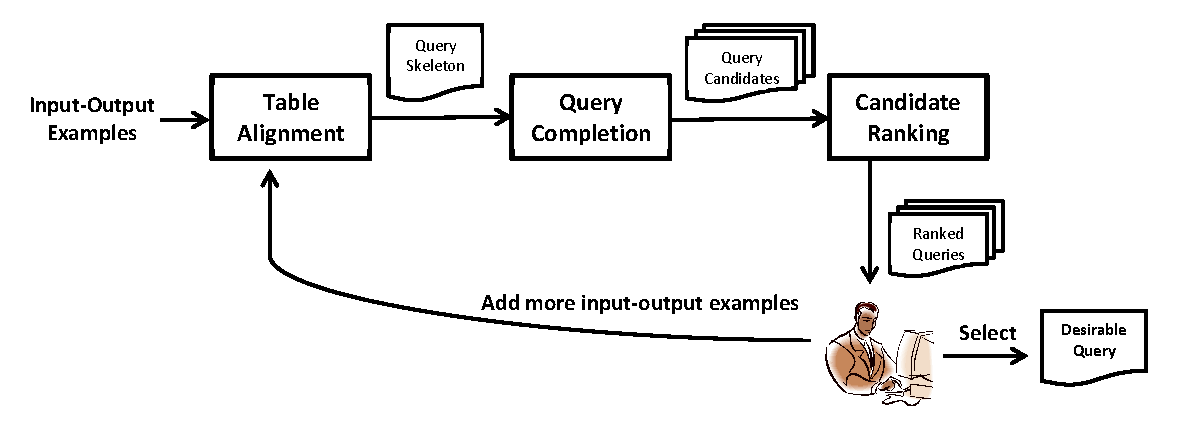
\includegraphics[scale=0.70]{workflow}
  \vspace*{-1.0ex}\caption {{\label{fig:workflow} Illustration
  of \ourtool's workflow of sythesizing SQL queries from input-output examples. 
}}

\end{figure*}

\subsection{Overview}
\label{sec:algorithm}

\vspace{-1mm}

Figure~\ref{fig:workflow} illustrates \ourtool's workflow.
\ourtool consists of three steps: (1) the ``Skeleton Creation'' step (Section~\ref{sec:skeleton})
creates a set of query skeletons from the given examples;
(2) the ``Query Completion'' step (Section~\ref{sec:completion}) 
infers the missing parts in each query skeleton and outputs
a list of syntactically-valid queries that satisfy
the provided example input and output; and (3) the ``Candidate Ranking'' step (Section~\ref{sec:ranking})
ranks all synthesized SQL queries and places the more likely ones near the top. 
Users can inspect the query list and select an expected query
from it.
If the synthesized SQL queries satisfy the example input and
output, but do not address the user's intention,
\ourtool can be used interactively by requesting more
informative examples from the end-user and then
update the result queries.\todo{xx}

Take the query in Figure~\ref{fig:queryex} as an example,
the ``Skeleton Creation''
step infers its projection columns, query tables, and join conditions; and
the ``Query Completion'' step infers the remaining parts (i.e., aggregates,
query conditions, the \CodeIn{GROUP BY} clause, the
\CodeIn{HAVING} clause, and the \CodeIn{ORDER BY} clause).

Figure~\ref{fig:algorithm} sketches \ourtool's high-level algorithm.
Line 2 corresponds to the first ``Query Skeleton
Creation'' step. Lines 3 -- 13 correspond to the second ``Query Completion''
step, in which \ourtool searches for the query conditions (line 4)\footnote{
Including conditions used in the \CodeIn{HAVIGN} clause.},
aggregates (line 5), and columns in the \CodeIn{ORDER BY} clause (line 6).
\ourtool then assembles a list of candidate SQL queries (line 7), and
validates their correctness on the examples (lines 8 -- 11).
Line 14 corresponds to the ``Query Ranking'' step.

%the result list (line 10). Finally, the query list is sorted by using
%the Occam's razor principle (line 14), and returned to the end-users.

\begin{figure}[t]

\textbf{Input}: example input table(s) $T_I$, example output table $T_O$\\

\vspace{-4mm}
\textbf{Output}: a ranked list of SQL queries\\
\vspace{1mm}
synthesizeSQLQueries({$T_{I}$, $T_{o}$})\\
\vspace{-5mm}
\begin{algorithmic}[1]
\STATE $\mathit{queryList}$ $\leftarrow$ an empty list\\
\STATE $\mathit{skeletons}$ $\leftarrow$ createQuerySkeletons($\mathit{T_I}$, $\mathit{T_O}$)
\FOR{each $\mathit{skeleton}$ in $\mathit{skeletons}$}
\STATE $\mathit{conds}$ $\leftarrow$ inferConditions($\mathit{T_I}$, $\mathit{T_O}$, $\mathit{skeleton}$)
\STATE $\mathit{aggs}$ $\leftarrow$ searchForAggregates($\mathit{T_I}$, $\mathit{T_O}$, $\mathit{skeleton}$, $conds$)
\STATE $\mathit{columns}$ $\leftarrow$ searchForOrderBys($\mathit{T_O}$, $\mathit{skeleton}$, $\mathit{aggs}$)
\STATE $\mathit{queries}$ $\leftarrow$ buildQueries($\mathit{skeleton}$, $\mathit{conds}$, $\mathit{aggs}$, $\mathit{columns}$)
\FOR{each $\mathit{query}$ in $\mathit{queries}$}
\IF{isValidOnExamples($\mathit{query}$, $\mathit{T_I}$, $\mathit{T_O}$)}
\STATE $\mathit{queryList}$.add($\mathit{query}$)
\ENDIF
\ENDFOR
\ENDFOR
\STATE rankQueries($\mathit{queryList}$)
\RETURN $\mathit{queryList}$
\end{algorithmic}
\vspace{-3mm}
\caption{Algorithm for synthesizing SQL queries from input-output examples.}
 \label{fig:algorithm}
\end{figure}


\subsection{Query Skeleton Creation}
\label{sec:skeleton}

%\todo{why need a skeleton. We divide the whole inference
%into three tasks}


A query skeleton is a partially-complete SQL query.
It consists of three parts: the tables used in
the query, the table columns used to join tables, and the table
columns used to project the query results.
Other elements in the query, such as query conditions
and aggregate functions, will be determined in
the next step.

A query skeleton captures the most basic structure of
a SQL query; creating it is the first step of sythesizing
a complete query. \ourtool performs a simple scan over
the examples, and employs several heuristics to determine
the table set, joining columns, and project columns.

\todo{why heuristics. the source of PSPACE}

%\item
\vspace{1mm}
{\textbf{Determining the Table Set.}} 
We observe that End-users are often unwilling to provide more than enough
input: every table in the example input
is expected to be used (at least once) in the result query.
Thus, we assume that every input table
should be used in the query. 
%By default, the table set contains all given input tables.
On the other hand, it is possible that one input table will be
used for multiple times in a query.
\ourtool does not forbid this case,
rather, it uses a heuristic
to estimate the table set: if one column from
an input table appears multiple times in the
example output, we add the input table to the table set the same
number of times.\todo{xx}

The rationale behind this heuristic is that if a table column
appears multiple times in the output, it may indiciate that the
table would be joined multiple times.



%\item
\vspace{1mm}
%\noindent
{\textbf{Determining the Joining Columns. }} Given a set of tables,
there are many ways to join them. Enumerating all possibilities
leads to a huge number of joining conditions and would quickly
become intractable. To make it feasible, we use
three simple but effective effective rules to capture
the most likely ways to join tables in practice.
%based We observe that, in practice, two tables are
%often joined via the following
%three cases: 
First, tables are often joined on their primary keys with
the same data type. For example, in Figure~\ref{fig:motivating},
the \CodeIn{student} table can be joined with the \CodeIn{enrolled}
table on the \CodeIn{student\_id} column.
By contrast, it is unlikely to join two tables on columns
with different types. Second, tables are often joined
on columns with the same name, since columns with the same name
often such as joining the \CodeIn{student} table
with the \CodeIn{enrolled} table on the
\CodeIn{student\_name} column. Third, it is only meaningful
to join two tables on columns that have the same data type and some
overlapped values. \todo{revise}

\ourtool restricts the search space in uses the above three rules \todo{need to revise}

%It is straightforward to check the first 
%two cases to identify possible joining columns. For the third case, our technique scans the given input tables to check ``value similarity''
%between two arbitrary columns, and selects columns whose ``value similarity'' is above a fixed threshold as joining columns.
\todo{need to implement above.}
\todo{mention how many skeletons will be created}
\todo{give an algorithm}

%\item
%\vspace{1mm}
%\noindent 
{\textbf{Determining the Output Columns.}} For each
column in the output table, \ourtool first checks whether
its column name appears in any of the input table.
If so, \ourtool uses the matched column from the input
table as the output column.
Otherwise, the output column
must be produced by using an aggregate function.
\todo{same names}
Consider the example in Figure~\ref{fig:motivating},
\ourtool determines that column {\CodeIn{name}} comes from the \CodeIn{student}
table, while column {\CodeIn{max\_Score}} must be created by using an aggregation operator.
\todo{If there is no column name}
%which the querying result would be projected, our technique checks whether each output
%table column name appears in any input tables. If so, we used the matched column
%from the input table as the output column.  Our technique keeps track of those aggregation columns
%and search for proper aggregates in the next phase (Section~\ref{sec:agg_search}). 
\todo{check the values in the output column}

\todo{It is possible that multiple skeleton can be created. add an algorithm here.}
\vspace{1mm}




\begin{figure}[t]
	\centering
		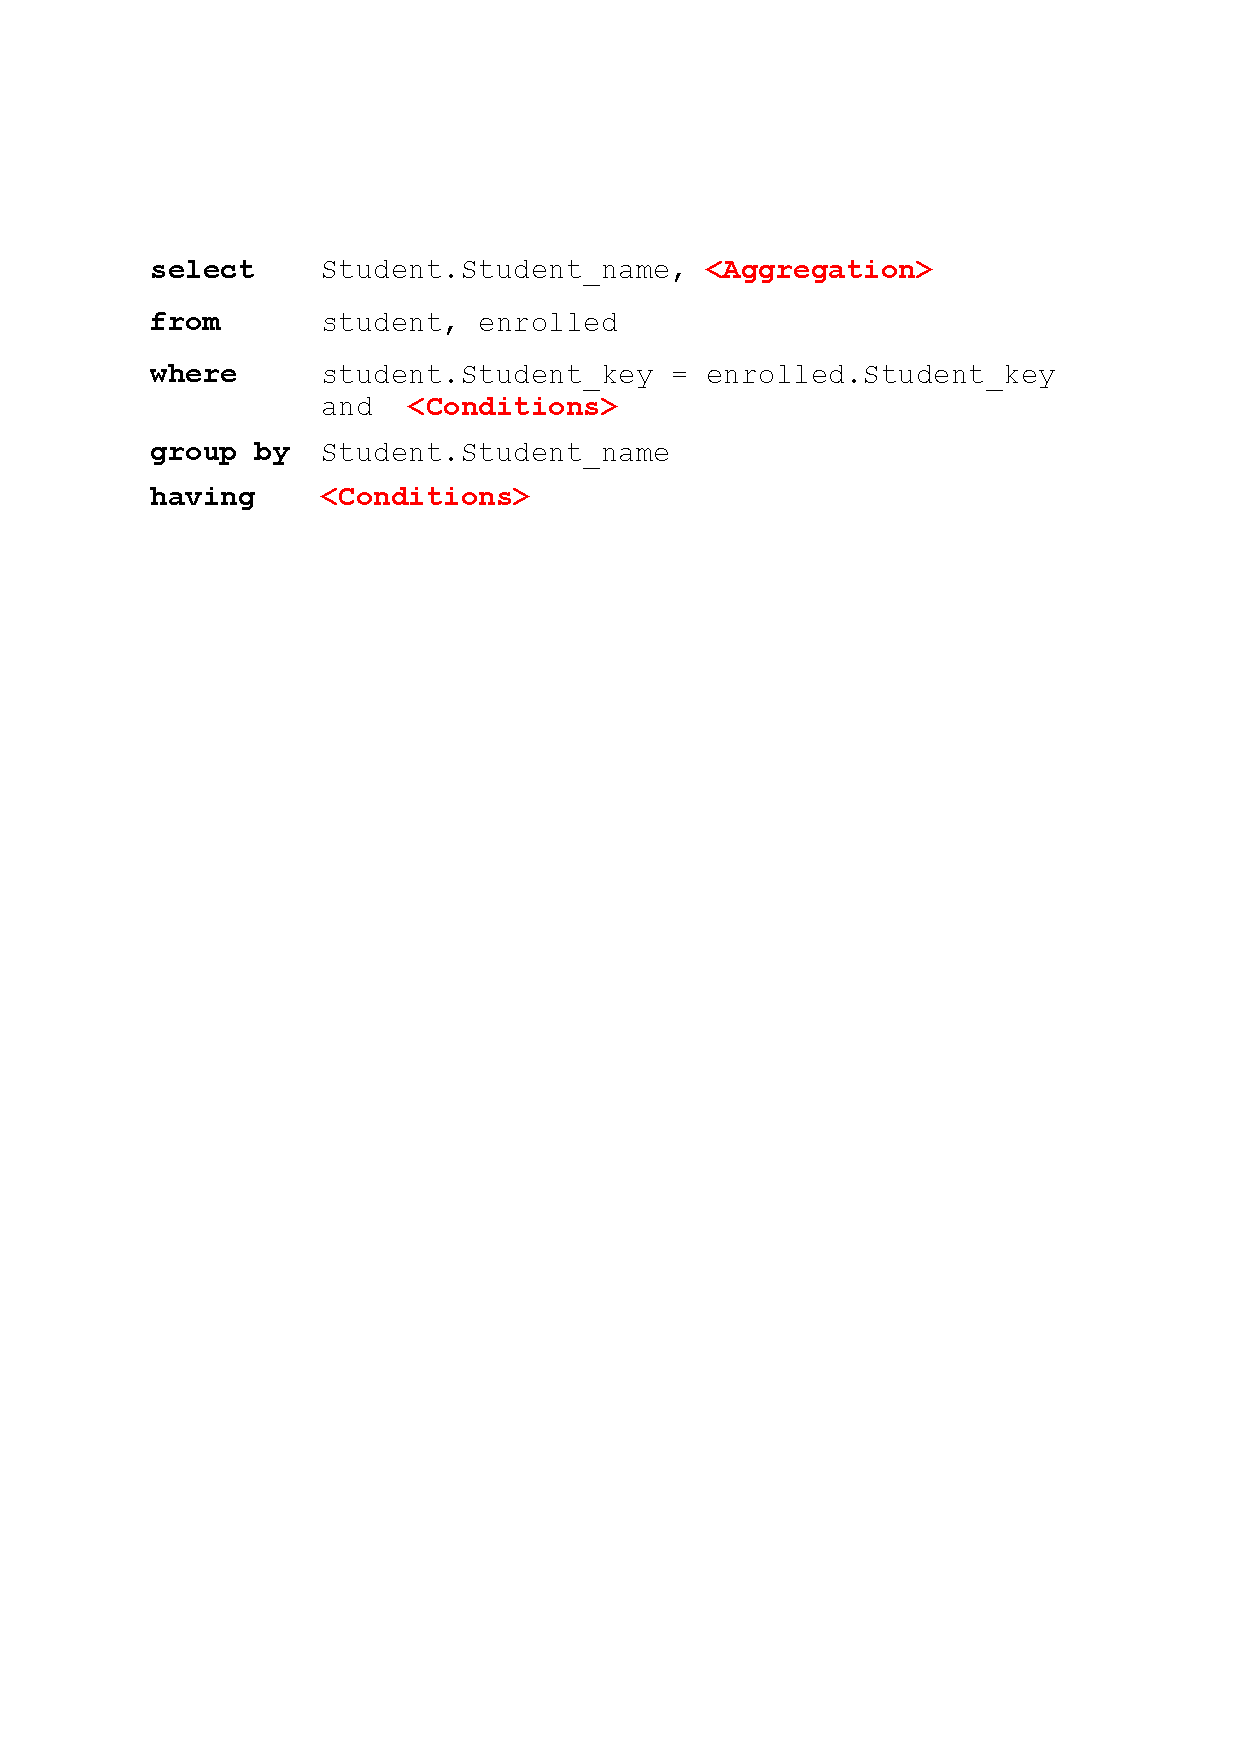
\includegraphics[width=0.45\textwidth]{sql_skeleton.pdf}
	\caption{The SQL skeleton created for the motivating example
in Figure~\ref{fig:motivating}.}
	\label{fig:skeleton}
\end{figure}

Figure~\ref{fig:skeleton} shows the created query skeleton
for the motivating example in Figure~\ref{fig:motivating}.
In this skeleton,  three unknown structures represented by
$<$Aggregation$>$ or $<$Conditions$>$ are in red, and
will be filled in the next phase. \todo{revise text}


\todo{how to create group by}

% which indicates aggregation and group by.

%After determining the table set and joining columns,
%the next step is to identify potential column names on which the result would be projected. If a
%column in the output table  does not appear in any input table's column list, this output column must
%be produced by aggregation. Our algorithm keeps track of these columns and appends a \CodeIn{group by} ... \CodeIn{having} ...
%clause to the query skeleton.

%\end{itemize}

%In summary, this step infers three parts as a query skeleton: tables used in constructing a SQL query, joining conditions
%to connect the input tables, and a list of columns to project the output results.

%It is worth noting that the results obtained from the above steps are not \textit{safe} in
%terms that they may miss some valid SQL queries. 

%We made the above assumption for the sake of tractability,
%since in theory, the bound of table number in a SQL query is $O(n_t!)$, where $n_t$ is the number of given tables;
%while the bound of possible number of join is $O(c_t^2)$ and the bound of the number of conditions is $O(n_t!n_tc_t^2)<O(n_t^3c_t^2)$.

%\subsubsection{Inferring Output Table Schema}

%Lacks schema


%while the bound of possible number of join is $O(c_t^2)$ and the bound of the number of conditions is $O(n_t!n_tc_t^2)<O(n_t^3c_t^2)$.




\subsection{Query Completion}
\label{sec:completion}

\begin{figure*}[t]
    \centering
    \includegraphics[scale=0.68]{featurex}
    \vspace{-7mm}
	\caption{Illustration of the two additional features
    added by \ourtool. (Left) An example input table with
    two columns: C1 and C2. (Center) The aggregation features added by
    \ourtool for the input table. (Right) The comparison features
    added by \ourtool for the input table.
    Take the first row in the input table as an example,
    when grouping by column C1 (with value 2), the number
    of tuples falling into that group is 3; the 
    distinct values in the C2 column is 2; the minimal value
    in the C2 column is 1, the maximal value in the C2 column
    is 4, and the average value in the C2 column is 2. Similarl
    results can be computed when the table is grouped by the C2
    column.
}
	\label{fig:features}
\end{figure*}


In this step, \ourtool analyzes each created query skeleton
, and completes the missing query conditions, the
\CodeIn{GROUP BY} and \CodeIn{HAVING} clause (Section~\ref{sec:condition}),
aggregates (Section~\ref{sec:agg_search}), and
the \CodeIn{ORDER BY} clause (Section~\ref{sec:orderby}).
\ourtool outputs a list of syntactically-correct SQL queries
that satisfy the given example input and output.


%The SQL skeleton produced by the first step, though incomplete,
%serves as a good reference in inferring complete and valid SQL queries.
%In this step, our technique the remaining incomplete parts: conditions and
%aggregates, by rule-based learning and type-directed search, respectively.

\subsubsection{Inferring Query Conditions}
\label{sec:condition}

\ourtool casts the problem of \textit{inferring query conditions} as
 \textit{learning appropriate rules} that can perfectly divide a search space
into a positive part and a negative part. In our context, the search space
is all tuples from joining all query tables; the positive part
includes all tuples in the output table; and the negative part includes the rest
tuples.

The standard way for rule learning is using a decision-tree-based
algorithm. However, how to design a good features
becomes a key challenge.
Existing approaches~\cite{Tran:2009} simply use
tuple values in the input table(s) as features, 
and limits their abilities in inferring more
complex rules as query conditions. In particular,
merely using tuple values as features can only infer
conditions that compares a column value with a constant
(e.g., \CodeIn{student.level = 'senior'}), but
fails to infer conditions using aggregates (e.g., \CodeIn{COUNT(enrolled.course\_id) > 2}),
or conditions comparing the values of two table columns
(e.g., \CodeIn{enrolled.course\_id > enrolled.score}).



\ourtool addresses this challenge by adding two types of
additional features to each tuple, and uses
the existing tuple values together with the additional features
for rule learning.

\begin{itemize}

\item {\textbf{Aggregation Features}}. For each
column in an input table, \ourtool tries
to group all table data by \textit{each} tuple's
value, then applies every applicable aggregate (i.e.,
\CodeIn{COUNT}, \CodeIn{COUNT DISTINCT}, \CodeIn{MAX},
\CodeIn{MIN}, and \CodeIn{AVG} for a numeric type column;
and \CodeIn{COUNT}, and \CodeIn{COUNT DISTINCT} for
a string type column) to every
 \textit{remaining} column for computing the aggregation result. 
The ``Aggregation Features'' part in Figure~\ref{fig:features}
shows an example.

\item {\textbf{Comparison Features}}. For each tuple,
\ourtool compares
the values of every two type-comparable columns, and records
the comparison results ($1$ or $0$) as features.
The ``Comparison Features'' part in Figure~\ref{fig:features}
shows an example.

\end{itemize}

%The above two additional features seamlessly encodes SQL
%structure
% knowledge encoding permits our technique
%to make use of correlations between columns, rather than only values
%from each isolated and sequential columns.
%Table~\ref{tbl:com} shows an example.


%Using both tuple values and the enhanced features,
\ourtool employs a variant of the decision tree algorithm,
called PART~\cite{Frank:1998}, to learn a set of rules
as query conditions.
PART has two notable advantages over the
original decision tree algorithm~\cite{Quinlan:1986}.
First, it uses a ``divide-and-conquer'' strategy to repeatedly
build rules and remove data instances (i.e., tuples) that have already been covered until
no more data instances are left, and thus is faster.
Second, PART less memory, since it builds a decision
tree incrementally, prunes falsified branches on-the-fly,
and only keeps the minimal tree structure in memory.



\todo{The incerasing number of features, can be falsified quickly,
more features permits undiscover more rules}


Figure~\ref{fig:fullexample} shows an example, in
which the expected query condition uses the \CodeIn{COUNT} aggregate.


\begin{figure*}[t]
  \centering
  \includegraphics[scale=0.65]{fullexample}
  \vspace*{-5.0ex}\caption {{\label{fig:fullexample}
  Illustration of how additional features added by \ourtool
  helps in inferring query conditions. (a) shows \ourtool
  enriches the original table (Left: the
  result of joining table \CodeIn{student} with table
  \CodeIn{enrolled} on the \CodeIn{student\_id} column)
  with additional features. For brevity, only relevant
  aggregation features are shown. Using the added aggregation
  features, \ourtool infers two query conditions that
  transform the original table into the table show in (b).
  Note that, without the aggregation features enhanced by
  \ourtool, a learning algorithm will \textit{fail} to learn the above conditions.
  (c) shows the output table, which is produced by projecting the
   table in (b)
  on its column: name, and an aggregate: \CodeIn{MAX}(score).
}}

\end{figure*}


\ourtool next splits the learnt rules into two disjoint parts:
and put each part into its appropriate place.
Specifically, \ourtool puts conditions
using aggregates to the \CodeIn{HAVING}
clause; and puts other conditions to the \CodeIn{WHERE} clause.
This is based on the SQL language's specification:
query conditions using aggregates are valid only when they
are used \textit{after} the \CodeIn{GROUP BY} clause.
Take the conditions inferred in Figure~\ref{fig:fullexample}
as an example, \ourtool puts the query
condition: \CodeIn{student.level =`senior'}
in the \CodeIn{WHERE} clause,
puts condition: \CodeIn{COUNT(enrolled.course\_id) > 2}
in the \CodeIn{HAVING} clause, and puts
column \CodeIn{student\_id} to the \CodeIn{GROUP BY} clause.

%\smallskip





%\end{itemize}

\subsubsection{Searching for Aggregates}
\label{sec:agg_search}

For every column in the output table that has no matched
column in the input tables,
\ourtool repeatedly applies each aggregate on
every input table column; and then outputs the aggregate (with the
input table column) that produces the same output 
in the output table. To speed up the exhaustive search,
\ourtool uses two rules to filter away many infeasible
combinations.


\begin{itemize}
\item \ourtool only applies an \textit{applicable} aggregate
to a \textit{type-compatible} table column. Specifically,
the data values in an output column must be compatible with an
aggregator's return type. For instance, if an output column
contains float values, it cannot be produced by using the \CodeIn{COUNT}
or \CodeIn{COUNT DISTINCT} aggregators, or 
using the \CodeIn{MAX} aggregator over a column with integer type.
On the other hand, some aggregates cannot be applied on
table columns with certain types. For example, the \CodeIn{AVG}
aggregate cannot be applied to columns with string type.
%\ourtool encodes such knowledge to avoid unnecessary search.

\item \ourtool checks whether each value in the output
column has appeared in the input table. If not, the
output column cannot be produced by using
using the \CodeIn{MAX} and \CodeIn{MIN} aggregator.
%such as \CodeIn{MAX} and \CodeIn{min},
%is used, each value in the output column must has appeared in the input table.
\end{itemize}

%In our experience, the type-directed searching strategy significantly reduces the
%searching space and makes our tool find the desirable aggregates faster.

%\todo{Order by structure, relatively each to add}
\subsubsection{Searching for columns in the \CodeIn{ORDER BY} column}
\label{sec:orderby}
\ourtool scans the values of each column in the output table. If
the data values in a column are sorted, \ourtool
append the column name to the \CodeIn{ORDER BY} clause.


\subsection{Candidate Ranking}
\label{sec:ranking}


It is possible that multiple SQL queries satisfying
the given input-output examples will be returned.
This may adversely impact end-users who want to
perform simple query tasks but now need
to select the query of their intent.
To alleviate this problem, we employ
the Occam's razor principle, which states that the
simplest explanation is usually the correct one, to
rank a more likely query higher in the output list.
A simpler query is less likely to overfit the given examples
than a complex query, even when both of them
can transform the example input to the example output.


%We define a comparison scheme between different
%SQL queries by defining a partial order between them. Some of
%these choices are subjective, but have been observed to work well.
A SQL query is simpler than another one if it uses
fewer query conditions (including conditions in the \CodeIn{Having}
and \CodeIn{from} clauses) or the expressions (including
aggregates) in each query condition are pairwise simpler
(e.g., expression \CodeIn{Count(student\_id)} is simpler than
\CodeIn{Count(Distinct student\_id)}.
Simpler query conditions suggests the extraction logics
are more common and general.

In our implementation, \ourtool computes a cost for each
query, and prefers queries with lower costs. The cost
for a SQL query is computing approximately by summarizing
the number of conditions, aggregates,
and other expressions
appearing in the \CodeIn{group by} and \CodeIn{order by} clauses.
This heuristic, though fairly simple, has been observed
to work well.
Figure~\ref{fig:rank} shows an example.


\begin{figure}[t]
\centering
 \includegraphics[scale=0.80]{rankexample}
 \vspace{-3mm}
\Caption{{\label{fig:rank} Illustration of \ourtool's
query candidate ranking heuristic. \ourtool produces two
queries for the given input-output examples. Based on
the heuristic in Section~\ref{sec:ranking}, the first query
differs from the second query by using simpler conditions,
and thus is ranks higher.
}}
\end{figure}




\subsection{Discussion}
\label{sec:uim}

%We next discuss some design issues in \ourtool.

\noindent \textbf{Soundness and Completeness.} The \ourtool
technique is neither sound nor complete. The primary
reason is that several steps (e.g., the Query Skeleton Creation
step in Section~\ref{sec:skeleton}) use heuristics
to infer possible joins, tables used in the \CodeIn{from} clause,
and columns in the \CodeIn{select} clause.
Such heuristics are necessary, since they provide a
good approximate solution to the problem of finding SQL queries
from examples, which has been proved to be
PSPACE-hard and is thus intractable in practice.
Although \ourtool cannot gurantee to infer correct SQL queries
for all cases, as demonstrated in Section~\ref{sec:evaluation},
we find \ourtool
is useful in sythesizing a wide variety of queries in practice.

\todo{no title}

\begin{comment}
\vspace{1mm}
\noindent \textbf{What if the input-output examples are not
representative enough?}
On some examples, \ourtool may produce a SQL query that
satisfies the input-output examples specified by the user,
but does not address the intention that the user wants.
To address this issue, we use a simple
interaction model~\cite{Harris:2011} to ask users to
investigate the query results and report any discrepancy.
After, the user can refine the inferred SQL query by providing a more
informative input-output example that demonstrate the behavior on
which the originally-inferred SQL query behaves incorrectly.
As demonstrated in our evaluation (Section~\ref{sec:evaluation}),
such an interactive model works fairly well in practice: 
a typical end-user only needs XXX rounds of interactions to
obtain the desirable SQL query.
\end{comment}


\vspace{-1mm}

\section{Implementation}
\label{sec:implementation}

We implemented the proposed technique in a tool, called \ourtool. 
\ourtool uses the Weka toolkit~\cite{Hall:2009}
to implement the rule-learning algorithm described in
Section~\ref{sec:completion}. \todo{inspect the above}

\ourtool uses MySQL~\cite{mysql} as the backend
database to check the correctness of each inferred
SQL query. Specifically, \ourtool populates the backend database
with the given input tables. When a SQL query is
synthesized, \ourtool executes the query on the database
to observe whether the output matches the given output.



\vspace{-1mm}

\section{Evaluation}
\label{sec:evaluation}

We evaluated four aspects of \ourtool's effectiveness,
answering the following research questions:

\begin{itemize}
\item What is the success ratio of \ourtool in sythesizing
a variety of SQL queries? (Section~\ref{sec:ratio}).
%Is the supported SQL subset expressive enough to describe a variety of queries?
\item How long does it take for \ourtool to
sythesize a SQL query (Section~\ref{sec:performance}).
\item How much human effort is needed to write sufficient
input-output examples for \ourtool in SQL sythesis (Section~\ref{sec:human}).
\item How does \ourtool's effectiveness compare to
an existing SQL query inference technique (Section~\ref{sec:comparison}).
\end{itemize}






\subsection{Benchmarks}

We collected benchmarks from two sources:

\begin{itemize}
\item We selected \textit{all} SQL query related exericses
(\allex in total) from a classic database textbook~\cite{cowbook}.
All exercises are from Chapter 5, which systematically
introduces the SQL language.
Exercises from a textbook are good resource to evaluate \ourtool's
generality, since such exericses are often designed to
cover a wide range of SQL features. Some exericses
are even designed on purpose to cover some less realistic,
corner cases in using SQL. As shown in Figure~\ref{tab:results},
each textbook exercises involves at least 3 tables. It was unintuitive
for us to write the correct query by simply looking at the problem
description in the exercise.

\item We searched SQL query related questions raised by real-world
database users from 3 popular online forums~\cite{stackoverflow, tutorialized, dbjournal}.
We focused on questions related to standard SQL features
rather than vendor-specific SQL features. We
excluded questions that were vaguely described or obviously
wrong, and discarded questions that had been proved
to be unsolvable by using SQL (e.g., computing a
transitive closure).
We collected \pnum forum questions related to writing a SQL query.
\todo{merge same types. exclude jdbc, why relative few}
\end{itemize}



\subsection{Evaluation Procedure}

We used \ourtool to solve each textbook exercise and forum
question. If an exericse or problem had
been associated with example input and output,
we directly applied \ourtool on the existing example.
Otherwise, we manually wrote some examples.
To reduce the bias in writing
examples, all examples are writting by a different graduate
student from University of Washington other than
\ourtool's developers.

We checked \ourtool's correctness by comparing its
output with the desired SQL queries. Specifically,
for textbook exericses, we compared \ourtool's output with
their correct answers, and for forum questions, we
manually determined whether the output query can fulfill
the query task or not.

For some textbook exercises and forum questions,
\ourtool inferred a SQL query that satisfied the input-output
examples, but did not behave as we expected when applied
to other inputs. We manually found another input on which the
SQL query mis-behaved and re-applied \ourtool to the new input. We
repeated this process and recorded the number of
interactions until \ourtool sythesized a desirable SQL query.


Our experiments were run on a 2.67GHz Intel Core PC
with 4GB physical memory (2GB was allocated for the JVM),
running Windows 7.


\begin{figure*}[t]
\setlength{\tabcolsep}{.24\tabcolsep}
\begin{tabular}{|c|c|c||c|c|c|c|c||l|}
\hline
\multicolumn{3}{|c||}{Benchmarks} & \multicolumn{5}{|c||}{\ourtool} & Query by\\
\cline{1-8}
 ID & Source & \#Input Tables & Example Size & Rank & Tool Cost (s) & Cost in Writing Examples (s) & \#Iterations & Output~\cite{Tran:2009}\\
 \hline
 \hline
 1 & Textbook Ex 5.1.1 & &  & & & & & \\
 1 & Textbook Ex 5.1.1 & &  & & & & & \\
 1 & Textbook Ex 5.1.1 & &  & & & & & \\
 1 & Textbook Ex 5.1.1 & &  & & & & & \\
 1 & Textbook Ex 5.1.1 & &  & & & & & \\
 1 & Textbook Ex 5.1.1 & &  & & & & & \\
 1 & Textbook Ex 5.1.1 & &  & & & & & \\
 1 & Textbook Ex 5.1.1 & &  & & & & & \\
 1 & Textbook Ex 5.1.1 & &  & & & & & \\
 1 & Textbook Ex 5.1.1 & &  & & & & & \\
 1 & Textbook Ex 5.1.1 & &  & & & & & \\
 1 & Textbook Ex 5.1.1 & &  & & & & & \\
 1 & Textbook Ex 5.1.1 & &  & & & & & \\
 1 & Textbook Ex 5.1.1 & &  & & & & & \\
 1 & Textbook Ex 5.1.1 & &  & & & & & \\
 1 & Textbook Ex 5.1.1 & &  & & & & & \\
 1 & Textbook Ex 5.1.1 & &  & & & & & \\
 1 & Textbook Ex 5.1.1 & &  & & & & & \\
 1 & Textbook Ex 5.1.1 & &  & & & & & \\
 1 & Textbook Ex 5.1.1 & &  & & & & & \\
 1 & Textbook Ex 5.1.1 & &  & & & & & \\
 1 & Textbook Ex 5.1.1 & &  & & & & & \\
 1 & Textbook Ex 5.1.1 & &  & & & & & \\
 1 & Textbook Ex 5.1.1 & &  & & & & & \\
 1 & Textbook Ex 5.1.1 & &  & & & & & \\
\hline
\end{tabular}
\Caption{{\label{tab:results} Experimental results in synthesizing SQL queries.
Column ``Benchmarks'' describes the characteristics of our benchmarks. Sub-column ``\#Input Tables''
shows the number of input tables in each benchmark. Column ``\ourtool'' shows
\ourtool's results in sythesizing SQL queries. Sub-column ``Example Size''
shows the number of rows in all example input and output tables.
Sub-column ``Rank'' shows the absolute
rank of the desirable SQL query in \ourtool's output. Sub-column ``Tool Time Cost (s)''
shows \todo{}. Sub-column ``\#Iterations'' shows the number of
interactive rounds in using \ourtool to obtain the desirable SQL query.
Column ``Query by Output'' shows the results of using a previous technique, called
\textit{Query by Output} (QBO)~\cite{}. Since \todo{treated as a special case},
we omit other. ``Y''  means QBO produces the desirable SQL queries, while ``N''
means QBO fails to produce the desirable SQL queries.
}}
\end{figure*}

\subsection{Results}

Figure~\ref{tab:results} summarizes our experimental results.

\subsubsection{Success Ratio}
\label{sec:ratio}


As shown in Figure~\ref{tab:results}, \ourtool
synthesized expected SQL queries for \solexnum  out of
\exnum the textbook exercises, and \solpnum out of
\pnum the forum questions.
%per exercise (or problem).

\todo{why the technique can work, why some problem
can not be solved}

%

\begin{figure*}[t]
  \centering
  \includegraphics[scale=0.70]{example2}
  \vspace*{-1.0ex}\caption {{\label{fig:example2} Input-output
  examples ((a) and (c)) taken from an online SQL help forum
  thread. \ourtool automatically sythensizes 6 SQL queries that
  can produce the output table from the three input tables.
  (b) shows the highest ranked SQL query.
}}
\end{figure*}

We use a real SQL question from
an online forum\footnote{\url{http://forums.tutorialized.com/sql-basics-113/join-problem-147856.html}} to illustrate
\ourtool's effectiveness.
The question was started by a novice user, who needed help to write a
SQL query to get result from three input tables. In this question, the
novice user described his required query in a few paragraphs of
English, but also include several small, representative input-output
examples as shown in Figure~\ref{fig:example2}, to better express
his intention. 
This question receives no replies as of April 2013 and we speculated that
writing a SQL query to join three tables to produce certain output results
is non-trivial.

We ran \ourtool on the input-output examples
in Figure~\ref{fig:example2}. The tool produced 6 valid answers
in less than 1 minutes, all of which satisfy the given examples. The
highest ranked SQL query is shown in Figure~\ref{fig:example2},
which is quite unintuitive to write. The SQL query in
Figure~\ref{fig:example2}
first joins three input tables
on columns \CodeIn{T1.Column2}, \CodeIn{T2.Column2},
\CodeIn{T2.Column1}, and \CodeIn{T3.Column1} using some
selected columns, and then aggregates the results based on
column \CodeIn{Table2.Column3}'s value. Finally, it
returns the minimal values of columns \CodeIn{T1.Column1}, \CodeIn{T1.Column4}, and \CodeIn{T3.Column2}
from each aggregated group as the results.




\subsubsection{Performance}
\label{sec:performance}

We measured \ourtool�s performance by recording the average
time cost in producing a ranked list of SQL queries. 
As shown in Figure~\ref{tab:results}, the performance of \ourtool is
reasonable. On average, it uses less than \avgtime minutes to
produce the results in one interative round.
Most of the time is spent querying the backend
database to validate the correctness of each sythesized SQL query.
%\todo{caching might be helpful}



\subsubsection{Human Efforts}
\label{sec:human}

We measured the human efforts taken to use \ourtool in two ways.
First, the time cost to write input-output examples. Second,
the number of interactive rounds in invoking \ourtool
to sythesize the desirable SQL queries.

As shown in Figure~\ref{tab:results}, human efforts
spent in providing input-output examples are very limited:
on average, it took less than 5 minutes for one benchmark.
\todo{explain some abnormal points}

The number of interactive rounds is a measure of
the generalization power of the conditional learning part
of the algorithm and the ranking scheme.
We observed that the tool typically requires
just \avground rounds of interaction, when the user is smart
enough to give an example for each input format (which
typically range from 1 to 3) to start with. This was indeed the case
for most cases in our benchmarks, even though our algorithm
can function robustly without this assumption. The maximum number
of interactive rounds required in any scenario was \todo{XXX}
(with 2 to 3 being a more typical number). \todo{the largest table}
The maximum number of examples
required in any scenario over all possible interactions was 10.

\subsubsection{Comparison with an Existing Technique}.
\label{sec:comparison}

We compared \ourtool with \textit{Query By Output} (QBO), a
data-driven approach to infer SQL queries~\cite{Tran:2009}. We chose
QBO because it is the most recent technique and also one
of the most precise SQL query inference techniques in
the literature. QBO requires similar input as \ourtool, and
uses a decision-tree-based algorithm
\todo{explaining what is QBO}
However, QBO cannot infer SQL queries using \todo{aggregates}

The experimental results of QBO is shown in Figure~\ref{tab:results}
(Column ``Query by Example''). For all \exnum database exercises
and \pnum forum questions, QBO produces correct answers
for XXX and XXX of them, respectively. QBO fails to
sythesize desirable SQL queries for other benchmarks, because
it \todo{the reasons}.

We did not compared \ourtool with other related techniques~\cite{},
for three reasons. \todo{reasons}

\subsection{Experimental Discussion}

\noindent \textbf{\textit{Limitations.}}
The experiments indicate three limitations
of our technique. First, the supported SQL
subset may not be expressive enough to write
database queries for certain tasks. \todo{not solved problems} As our
future work, we plan to include more SQL features
to the supported subset, and improve the current
sythesis algorithm.
Second, on some examples, the learned query
condition, though correct, may not be accurate; and requires
users to provide more informative examples.
Take the example input and output in Figure~\ref{fig:rank}
as an example, \ourtool produces a SQL
query \CodeIn{select name from student where score > 3}
\todo{exam}
which perfectly satisify the examples. However, if
the query conditoin of the desirable SQL query
should be \CodeIn{score > 2}, users must provide
one more record in the input table with score 3 
to guide \ourtool to learn the correct query condition.
Third, \ourtool requires
users to provide noise-free input-output examples.
Even in the presence of a small amount of user-input
noises (e.g., a typo), \ourtool will declare failure
when it fails to infer a valid SQL query.
To overcome this limitation, we plan to design a more
robust inference algorithm that can attempt to identify
and tolerate user-input noises, and even suggest a fix
to the noisy example.

\vspace{1mm}
\noindent \textbf{\textit{Threats to Validity.}}
There are three major threats to validity
in our evaluation. First, the \exnum textbook exercises
and \pnum forum questions, though covering
a wide variety of SQL features, may not be representative enough.
Thus, we can not claim the results can be generalized to an
arbitrary scenario. Second, we only compared
\ourtool with the \textit{Query by Output} technique~\cite{Tran:2009}.
Using other query inference or recommendation techniques
might achieve different results. Third, our
experiments focus on evaluating \ourtool's generality 
and accuracy. Even though all experiments are carried
out by a different person other than \ourtool's developers,
it is unknown about \ourtool's general usability for other
end-users. To address this issue, we plan to conduct
a user study in our future work.


\vspace{1mm}
\noindent \textbf{\textit{Experimental Conclusions.}}
We have three chief findings: \textbf{(1)}
The supported SQL subset in \ourtool is
expressive enough to describe a variety of database queries.
\textbf{(2)} \ourtool can efficiently synthesize desirable SQL
queries with a small amount of human
efforts and small input-output examples.
\textbf{(3)} \ourtool produces better results
than an existing technique (\textit{Query by Output}~\cite{Tran:2009}).






\vspace{-1mm}

\section{Related Work}
\label{sec:related}

This section discusses two categories
of closely-related work on reverse query processing 
and automated program synthesis.


\subsection{Reverse Query Processing}

In the database community, there is a rich body of
work~\cite{Zloof:1975, Tran:2009, DasSarma:2010} that share the same broad principle
of ``reverse query processing''. Zloof's work on \textit{Query by Example} (QBE)
~\cite{Zloof:1975} provided an intuitive form-based Graphical User Interface for
writing database queries, which is completely different than ours.
\todo{add why it is different}



Tran et al.~\cite{Tran:2009} studied the problem of \textit{Query By Output} (QBO). 
The problem of QBO is similar to the view synthesis problem, but the technique
presented in~\cite{Tran:2009} infers simple select-project-join queries.
Of the examples presented in this paper, such queries can only be applied
to satisfy the example in \todo{some example}, and such queries cannot
be applied to many of the other real-world cases that we studied (Section~\ref{}).
The key limitation of \todo{fail to encode extra features}


Recently, Sarma et al.~\cite{DasSarma:2010} proposed a technique
to address the \textit{View Definitions Problem} (VDP).
\todo{explain more here}
With a rather different goal than \ourtool,
VDP aims to to find the most succinct and accurate view definition, when
the view query is restricted to a specific family of queries.
VDP can be treated as a special
case of QBO where $n = 1$ and there are no joins nor projections.
Compared to \ourtool, there are three key differences:
(1) VDP aims to infer a relation from a large representative
example view, while \ourtool attempts to infer a SQL query from a
set of few input-output examples \todo{revise below}
(which is a critical usability aspect for end-users who lack adequate
SQL experience). (2) the technique proposed by Sarma et al.~\cite{DasSarma:2010} does
not consider join or projection
operations and assumes the output view to be a strict subset of the input
database with the same schema\todo{revise}, while our work eliminates these
assumptions, and considers both join and projection operations.\todo{revise above}



\todo{what is the limitation of non program sythesis, why
sythensis would be useful.}

\subsection{Automated Program Synthesis }


Program synthesis~\cite{Gulwani:2010:DPS} aims to create an executable program
in some underlying language from specifications that can range
from logical declarative specifications to examples or
demonstrations~\cite{Harris:2011, singh:2012, Gulwani:2011,
Kandel:2011, Fisher08Pads,Lau:2003:PDU, Lau:2000:VSA, Barbosa:2010:MLA, Arasu:2009:LST}.

Automated program synthesis techniques 
has been used recently for many applications
such as synthesis of efficient low-level code~\cite{Solar-Lezama:2005},
data structure manipulations~\cite{Fisher:2008},
geometry constructions~\cite{Gulwani:2011:SGC},
snippets of excel macros~\cite{Harris:2011},
relational data representations~\cite{Barbosa:2010:MLA, Arasu:2009:LST} and string
expressions~\cite{singh:2012, Gulwani:2011}.


PADS~\cite{Fisher:2008} takes a large sample of unstructured data and infers a
format that describes the data. Users then manually define tools for
data in the format.
Though well-suited for their intended tasks, these
systems are insufficient for the database query tasks.
For example, while text extraction and mass editing
are quite valuable for data transformation, the above tools
lack other needed operations such as table
re-shaping, aggregation, and missing value imputation.
\todo{explain}


Closely related to our current work is Harris and Gulwani�s
system for learning excel spreadsheet transformations
from an example input-output pair~\cite{Harris:2011}. Given input and output
tables, their system can infer an excel macro that filters,
duplicates, and/or reorganizes table cells to generate the output table.
These resulting programs can express a variety of table
re-shaping operations. \ourtool differs in multiple respects.
First, Harris and Gulwani's approach treats table cells
as atomic units, and thus has limited expressiveness.
For example, it does not support queries involving text editing or extraction\todo{xxx}.
Second, \todo{explain the difference between excel work}


The Wrangler tool, developed in the HCI community, provides a nice visual
programming-by-demonstration interface to table transformations
for data cleaning~\cite{Kandel:2011}. By contrast, \ourtool provides
an interface based on examples, which is more
friendly to end users. \todo{xxx}


There is some recent work for inferring SQL queries for database end-users.
Query recommendation systems, such as SQLShare~\cite{} and SQLSnippet~\cite{},
\todo{explain}
may achieve a similar goal of helping end-users write better SQL
queries, but they rely on information
that we cannot assume access to in many realistic scenarios: a query log~\cite{Khoussainova:2010},
or user history and preferences~\cite{Howe:2011}.

Cheung et al~\cite{abs-1208-2013} presented a technique to infer SQL
queries from imperative code.
Their technique automatically identifies
fragments of application logic (written in an imperative language
like Java) that can be pushed into
SQL queries. 
\todo{focus on performance...}

%also cite this~\cite{Cheung:2012:UPS}, combining machine learning with program synthesis.


\section{Conclusions and Future Work}
\label{sec:conclusion}

Sai will write this section




\vspace{-1mm}

\section{Acknowledgement}

We thank Dan Suciu, Michael Ernst and Hao L{\"u} for their insightful comments
on an initial draft. This
work was supported in part by NSF grants
CCF-1016701 and CCF-0963757.

%\balance

%\bibliographystyle{plain}
%\bibliography{sqlsynthesis}

%\begin{multicols}{2}
%\bibliographystyle{IEEEtran}
\bibliographystyle{plain}
\bibliography{sqlsynthesis}
%\end{multicols}

\end{document}
